\documentclass{article}
\usepackage{amsmath}
\usepackage{amssymb}
\usepackage{graphicx}
\usepackage{hyperref}
\usepackage[version=4]{mhchem}

\title{Example 3}
\date{}

\begin{document}
\maketitle

(AMC) In triangle \(A B C\) the ratio \(A C: C B\) is 3:4. The bisector of the exterior angle at \(C\) intersects \(B A\) extended at \(P(A\) is between \(P\) and \(B\) ). The ratio \(P A: A B\) is:\\
(A) \(1: 3\)\\
(B) \(3: 4\)\\
(C) \(4: 3\)\\
(D) \(3: 1\)\\
(E) \(7: 1\)

Solution: (D).\\
\centering
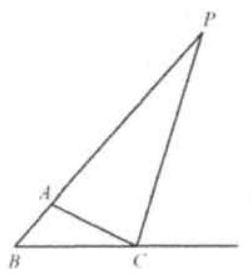
\includegraphics[width=\textwidth]{images/problem_image_1.jpg}


Draw \(P A^{\prime}\) such that \(\angle B P C=\angle A^{\prime} P C\), then \(\triangle A C P \cong \triangle A^{\prime}\) \(C P\) (ASA) and \(A C=A^{\prime} C, P A=P A^{\prime}\). Since \(P C\) bisects \(\angle B P A^{\prime}\) in \(\triangle B P A^{\prime}\),\\
\(\frac{B C}{C A^{\prime}}=\frac{P B}{P A^{\prime}}\) or \(\frac{B C}{C A}=\frac{P B}{P A}=\frac{4}{3}\).\\
\(A B=P B-P A\) since \(A\) is between \(P\) and \(B\).\\
\centering
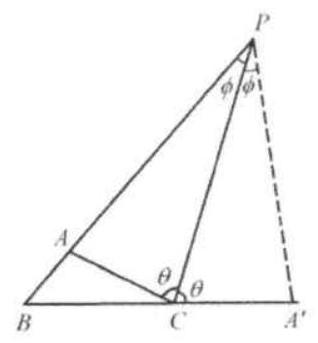
\includegraphics[width=\textwidth]{images/reasoning_image_1.jpg}\\
\(\frac{A B}{P A}=\frac{P B}{P A}-\frac{P A}{P A}=\frac{4}{3}-1=\frac{1}{3}\), so \(\frac{P A}{A B}=\frac{3}{1}\).\\

\end{document}
